\documentclass[runningheads]{llncs}

\usepackage[T1]{fontenc}
\IfFileExists{newtxtext.sty}{%
  \usepackage{newtxtext}
}{%
  \usepackage{times}
}
\usepackage{tikz}
\usetikzlibrary{arrows.meta,positioning,fit}
\usepackage{booktabs}
\usepackage{multirow}
\usepackage{makecell}
\usepackage{graphicx}
\graphicspath{{images/}}
\usepackage{amsmath,amssymb,amsfonts}
\IfFileExists{newtxmath.sty}{\usepackage{newtxmath}}{}
\usepackage{textcomp}
\usepackage{xcolor}
\usepackage{enumitem}
\setlist{noitemsep,topsep=2pt,leftmargin=*}

\tikzset{
  block/.style={draw, rounded corners=2pt, align=center, minimum height=7mm,
    inner xsep=4pt, font=\scriptsize, fill=gray!8},
  smallblock/.style={draw, rounded corners=2pt, align=center, minimum height=6mm,
    inner xsep=3pt, font=\scriptsize, fill=blue!7},
  loss/.style={draw, rounded corners=2pt, align=center, minimum height=6mm,
    inner xsep=4pt, font=\scriptsize, fill=orange!12},
  arr/.style={-{Latex[length=2mm]}, line width=.35pt}
}

\begin{document}

\title{Curriculum-Guided Siamese Real-ESRGAN with High-Order Degradation for Real-World Image Super-Resolution}
\titlerunning{Curriculum-Guided Siamese Real-ESRGAN for Real-World Image Super-Resolution}

\author{LE Hoai Nam\inst{1} \and NGUYEN Hoang Ha\inst{1}\thanks{Corresponding author.}}
\authorrunning{L. H. Nam and N. H. Ha}

\institute{University of Science and Technology of Hanoi, Vietnam Academy of Science and Technology, Hanoi, Vietnam\\
\email{nguyen-hoang.ha@usth.edu.vn}}

\maketitle

\begin{abstract}
Real-world image degradation combines blur, sensor noise, chromatic aberration, and JPEG compression, making synthetic restoration training difficult. We present a Siamese Real-ESRGAN framework that improves degradation diversity and training stability for realistic image restoration. The method extends high-order degradation with probabilistic operation selection, tuned compression ranges, camera-noise simulation, and offline multi-level quality generation. A shared-weight Teacher--Student training scheme restores paired inputs with different degradation severity, while a three-stage curriculum gradually shifts from mild to severe degradation pairs. Experiments on standard and real-world benchmarks show improved perceptual quality, reaching NIQE 3.82 on Urban100 and an 18.7\% NIQE gain over Real-ESRGAN on RealSR Canon, without increasing inference cost.

\keywords{Image Super-Resolution \and Siamese Network \and Knowledge Distillation \and Realistic Degradation \and Real-ESRGAN}
\end{abstract}

\section{Introduction}

Single-image super-resolution (SR) recovers high-quality images from low-quality observations. Deep SR methods perform well under bicubic degradation, but real photographs contain mixed artifacts from optics, sensors, compression, and post-processing. ESRGAN~\cite{wang2018esrgan}, BSRGAN~\cite{zhang2021designing}, and Real-ESRGAN~\cite{wang2021realesrgan} improve perceptual blind SR, yet a single degradation distribution remains insufficient for severe or differently ordered real artifacts.

This work extends our previous Real-ESRGAN refinement study~\cite{11309534}. That work improved degradation synthesis and conventional distillation for compression. Here, we target robust restoration under gradually increasing degradation severity. Instead of a fixed large Teacher and a separate Student, one shared-weight generator runs two passes: the milder input guides the harder one, and the curriculum moves both inputs toward stronger degradation levels. We make three main contributions. First, we introduce a shared-weight Siamese Real-ESRGAN training scheme that requires no additional parameters at inference time. Second, we design a three-stage curriculum (90\%/80\%, 80\%/70\%, and 70\%/60\%) to stabilize training under progressively severe degradations. Third, we develop an enhanced high-order degradation pipeline with probabilistic operation ordering, realistic JPEG compression, camera noise simulation, and offline multi-level data generation.

\section{Related Work}

 SRCNN~\cite{dong2014learning}, EDSR~\cite{lim2017enhanced}, and RDN~\cite{zhang2018residualdensenetworkimage} advanced deep SR but mostly assume bicubic degradation. Blind SR methods~\cite{zhang2018learning,luo2020unfolding,gu2019blind} model unknown degradations, while Real-ESRGAN~\cite{wang2021realesrgan} uses high-order synthetic degradation. We build on it directly, but generate four offline quality levels for curriculum pairing. Knowledge Distillation (KD)~\cite{hinton2015distilling,Hui_2019} usually uses a fixed Teacher; feature-aware variants such as FAKD~\cite{gao2022featuredistillationinteractionweighting} preserve structure similarly. In contrast, Siamese networks~\cite{bromley1993signature,koch2015siamese} learn from paired inputs under shared weights, matching our paired degradation levels. Curriculum learning~\cite{bengio2009curriculum,soviany2022curriculum} motivates the easy-to-hard schedule. Recent diffusion SR models~\cite{wang2024exploiting,lin2023diffbir,yang2023pixel} are strong but costly, so we keep a practical GAN-based backbone.

\section{Methodology}
The proposed framework has two components: multi-level realistic degradation and weight-sharing Siamese training. Fig.~\ref{fig:overview} summarizes the full pipeline, which extends the degradation design from our previous work~\cite{11309534}.
\begin{figure}[t]
\centering
\resizebox{\textwidth}{!}{%
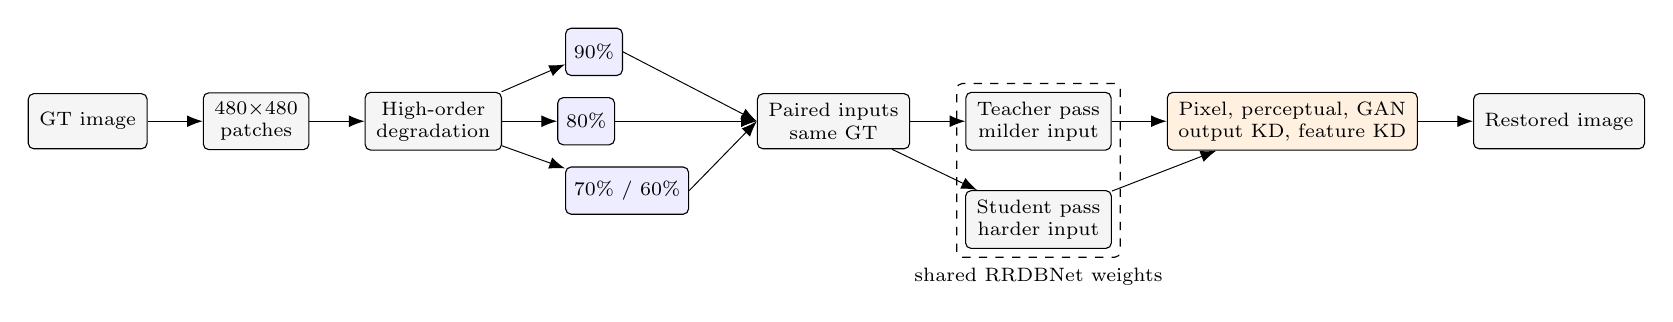
\begin{tikzpicture}[node distance=4.5mm and 7mm]
  \node[block] (gt) {GT image};
  \node[block, right=of gt] (crop) {$480{\times}480$\\patches};
  \node[block, right=of crop] (deg) {High-order\\degradation};
  \node[smallblock, above right=2mm and 8mm of deg] (q90) {90\%};
  \node[smallblock, right=of deg] (q80) {80\%};
  \node[smallblock, below right=2mm and 8mm of deg] (q70) {70\% / 60\%};
  \node[block, right=18mm of q80] (pair) {Paired inputs\\same GT};
  \node[block, right=of pair] (teacher) {Teacher pass\\milder input};
  \node[block, below=5mm of teacher] (student) {Student pass\\harder input};
  \node[loss, right=of teacher] (loss) {Pixel, perceptual, GAN\\output KD, feature KD};
  \node[block, right=of loss] (sr) {Restored image};

  \draw[arr] (gt) -- (crop);
  \draw[arr] (crop) -- (deg);
  \draw[arr] (deg) -- (q90);
  \draw[arr] (deg) -- (q80);
  \draw[arr] (deg) -- (q70);
  \draw[arr] (q90.east) -- (pair.west);
  \draw[arr] (q80.east) -- (pair.west);
  \draw[arr] (q70.east) -- (pair.west);
  \draw[arr] (pair) -- (teacher);
  \draw[arr] (pair) -- (student);
  \draw[arr] (teacher) -- (loss);
  \draw[arr] (student) -- (loss);
  \draw[arr] (loss) -- (sr);
  \node[draw, dashed, rounded corners=2pt, fit=(teacher)(student), inner sep=3pt,
        label={[font=\scriptsize]below:shared RRDBNet weights}] {};
\end{tikzpicture}}
\caption{Overview of the proposed Siamese Real-ESRGAN framework. Multi-level degraded samples are paired by curriculum stage and processed by one shared-weight generator in two passes.}
\label{fig:overview}
\end{figure}

\subsection{Multi-Level High-Order Degradation}

Real-ESRGAN synthesizes low-quality images through resizing, blur, noise, and JPEG compression. Following our previous degradation pipeline~\cite{11309534}, we keep the two-stage structure but add probabilistic operation selection, practical JPEG ranges, and camera-specific noise including chromatic aberration and sensor shot/read noise.

For an HQ image $I_{HQ}$, the generated LQ image at quality level $q$ is formulated as
\[
I_{LQ}^{(q)} = \mathcal{D}_{q}(I_{HQ})
= \Pi\big(R_{0.25}, B_{\Theta_q}, N_{\Theta_q}, C, J_{\Theta_q}\big)(I_{HQ}),
\]
where $R$, $B$, $N$, $J$, and $C$ denote resizing, blur, noise, JPEG compression, and camera-specific noise. The resize factor is fixed to $0.25$ for $\times4$ SR. $\Pi(\cdot)$ follows the implementation: resize is kept first in the first pass; blur, noise, camera noise, and JPEG are then sampled by probability, and a second pass applies the selected non-resize degradations. The level $q\in\{90,80,70,60\}$ is a quality index, not an evaluation score: $q=100$ is the original GT image, larger $q$ is milder, and lower $q$ is stronger.

In our implementation, each level changes the parameter set
\[
\Theta_q=(\Sigma_q,Q_q,p^B_q),
\]
where $\Sigma_q$ is the Gaussian-noise sigma range, $Q_q$ is the JPEG quality range, and $p^B_q$ is the blur probability:
\[
\begin{array}{c|c|c|c}
q & \Sigma_q & Q_q & p^B_q \\
\hline
90 & [1,10] & [75,95] & 0.4\\
80 & [5,15] & [60,85] & 0.6\\
70 & [10,20] & [45,70] & 0.7\\
60 & [15,25] & [30,55] & 0.8
\end{array}
\]
The remaining generator probabilities are shared across levels ($p^{resize}=1.0$, $p^{noise}=0.9$, $p^{JPEG}=0.9$, and $p^{camera}=0.7$). Thus, 90\% samples preserve more structure through weaker noise, lighter compression, and lower blur probability, while 60\% samples contain stronger noise, heavier JPEG artifacts, and more frequent blur.

\begin{figure}[t]
\centering
\includegraphics[width=\textwidth]{Realdegradationstructure.png}
\caption{Enhanced two-stage realistic degradation pipeline inherited and extended from our previous work~\cite{11309534}.}
\label{fig:degradation}
\end{figure}

For $\times4$ SR, GT images are cropped into $480\times480$ patches with 50\% overlap, producing $120\times120$ LQ counterparts. Each patch is pre-degraded into the four levels above, enabling efficient and reproducible 90/80, 80/70, and 70/60 pairing.

\subsection{Siamese Training with Shared Weights}

The generator is the Real-ESRGAN RRDBNet backbone~\cite{wang2018esrgan,wang2021realesrgan} with 23 RRDB blocks and 64 feature channels. Each mini-batch contains two degraded versions of the same GT image. The milder Teacher pass runs under \texttt{torch.no\_grad()} and produces $T_{HQ}$ and $T_{feat}$; the harder Student pass produces $S_{HQ}$ and $S_{feat}$. Both passes share weights, and only the Student pass receives gradients.

\IfFileExists{images/student_teacher_siamese.drawio.png}{%
\begin{figure}[t]
\centering
\includegraphics[width=\textwidth]{student_teacher_siamese.drawio.png}
\caption{Weight-sharing Siamese training architecture. Teacher and Student passes share the same generator parameters; only the Student pass receives gradient updates.}
\label{fig:siamese_architecture}
\end{figure}
}{}

The training objective combines reconstruction, perceptual, adversarial, and consistency losses:
\[
L_{total}=w_{pix}L_{pix}+w_{per}L_{per}+w_{GAN}L_{GAN}
\;+\lambda^{out}_{kd}L^{out}_{kd}+\lambda^{feat}_{kd}L^{feat}_{kd}.
\]
$L_{pix}$ is L1 loss to GT, $L_{per}$ is VGG19 perceptual loss~\cite{simonyan2014very,johnson2016perceptual}, and $L_{GAN}$ uses a spectral-normalized U-Net discriminator. $L^{out}_{kd}$ and $L^{feat}_{kd}$ align Student outputs and features with detached Teacher targets, giving dynamic guidance without a second stored network.

\subsection{Curriculum Schedule}

Training uses three phases: 90\%/80\% for stable warm-up, 80\%/70\% for the best perceptual balance, and 70\%/60\% for severe-degradation robustness. Since 100\% denotes GT, the first value in each pair is the milder Teacher input and the second value is the harder Student input. The pairwise gap remains 10 percentage points, while the absolute degradation severity increases from Phase~1 to Phase~3.

\section{Experiments}

\subsection{Experimental Setup}

Training uses the same sources as our previous work~\cite{11309534}: DF2K, Unsplash, and RealSR. Only HQ images are retained; all LQ images are generated by our degradation pipeline. Unlike bicubic pairs, our data combines multi-stage blur, resizing, noise, camera artifacts, compression, probabilistic operations, and multiple severity levels. This better approximates real acquisition but makes pixel-faithful reconstruction harder. Evaluation uses Set5, Set14, RealSR Canon/Nikon, BSDS100, and Urban100.

We report PSNR, SSIM, and NIQE~\cite{mittal2012making}. PSNR/SSIM measure distortion fidelity, while lower NIQE indicates better naturalness and is often more relevant for real-world SR~\cite{wang2021realesrgan}. Training follows Real-ESRGAN with Adam, learning rate $1\times10^{-4}$, 800k iterations, 10k warm-up, and MultiStepLR decay at 200k, 400k, 500k, and 700k. Loss weights are $w_{pix}=2.0$, $w_{GAN}=0.5$, and $\lambda^{out}_{kd}=\lambda^{feat}_{kd}=0.15$. Experiments run on an RTX 3090; inference remains comparable to Real-ESRGAN because the 16.7M-parameter backbone is shared.

\subsection{Quantitative Results}

Table~\ref{tab:quantitative_results} focuses on Real-ESRGAN variants to make the comparison fair and attributable. The original Real-ESRGAN row reports the released model trained with Real-ESRGAN's online high-order degradation setting. In contrast, our variants use a pre-generated multi-level degradation setting: each HR image is converted into controlled 90\%, 80\%, 70\%, and 60\% LQ versions, which enables fixed mild-to-hard pairs for Siamese curriculum training. The \textit{Real-ESRGAN with Multi-level Degradation} row isolates the degradation-setting effect without Siamese training: it improves PSNR/SSIM on RealSR Canon/Nikon and BSDS100, but high NIQE shows that richer degradation alone does not guarantee perceptually natural restoration. With Siamese curriculum learning, Phase~2 reaches NIQE 3.82 on Urban100 and reduces RealSR\_V3 Canon NIQE from 7.02 to 5.71, an 18.7\% gain. Phase~3 further improves NIQE on RealSR Canon/Nikon and Set14, at the cost of lower PSNR/SSIM due to stronger degradation.

\begin{table*}[t]
\centering
\caption{Comparison of Real-ESRGAN variants on benchmark datasets. The original row uses the released Real-ESRGAN model with online high-order degradation; all other rows use our generated multi-level degradation setting.}
\label{tab:quantitative_results}
\renewcommand{\arraystretch}{1.1}
\resizebox{\textwidth}{!}{%
\begin{tabular}{llccccccccccccc}
\toprule
\multirow{2}{*}{\textbf{Model}} & \multirow{2}{*}{\makecell{\textbf{Degradation} \\ \textbf{Setting}}} 
  & \multicolumn{2}{c}{\textbf{Set5}} 
  & \multicolumn{2}{c}{\textbf{Set14}} 
  & \multicolumn{2}{c}{\textbf{RealSR\_V3 (Canon)}} 
  & \multicolumn{2}{c}{\textbf{RealSR\_V3 (Nikon)}} 
  & \multicolumn{2}{c}{\textbf{BSDS100}} 
  & \multicolumn{2}{c}{\textbf{Urban100}}
  & \multirow{2}{*}{\makecell{\textbf{Avg.} \\ \textbf{Time (s)}}} \\
\cmidrule(lr){3-4}\cmidrule(lr){5-6}\cmidrule(lr){7-8}\cmidrule(lr){9-10}\cmidrule(lr){11-12}\cmidrule(lr){13-14}
 & & \textbf{PSNR/SSIM} & \textbf{NIQE} 
   & \textbf{PSNR/SSIM} & \textbf{NIQE} 
   & \textbf{PSNR/SSIM} & \textbf{NIQE} 
   & \textbf{PSNR/SSIM} & \textbf{NIQE} 
   & \textbf{PSNR/SSIM} & \textbf{NIQE} 
   & \textbf{PSNR/SSIM} & \textbf{NIQE} & \\
\midrule

Real-ESRGAN~\cite{wang2021realesrgan}
  & Original online
  & \textbf{26.31}/\textbf{0.80}            & 7.89
  & \textbf{25.18}/\textbf{0.69}            & 5.88
  & 25.84/0.78                              & 7.02
  & 25.19/0.75                              & 6.69
  & 22.34/0.57                              & 4.46
  & \textbf{20.12}/\textbf{0.64}            & 4.35
  & 1.55 \\

\makecell[l]{Real-ESRGAN }
  & Multi-level
  & 24.40/0.67                         & 10.44
  & 24.52/0.67                           & 6.10
  & \textbf{27.55}/\textbf{0.81}         & 7.05
  & \textbf{26.24}/\textbf{0.77}         & 6.94
  & \textbf{22.49}/\textbf{0.58}         & 4.83
  & 20.06/0.61                          & 4.33
  & \textbf{1.35} \\

\makecell[l]{\textbf{Real-ESRGAN} \\ \textbf{student (Ours)}}
  & Multi-level
  & 25.19/0.76                              & \textbf{6.54}
  & 23.89/0.69                              & 5.82
  & 26.77/0.80                              & 6.78
  & 25.93/0.76                             & 6.25
  & 22.31/0.57                             & 4.82
  & 20.00/0.59                              & 4.05
  & 1.45 \\

\makecell[l]{\textbf{Real-ESRGAN} \\ \textbf{siamese (Ours)} \\ \textbf{Phase 2}}
  & 80\%/70\%
  & 23.37/0.71                              & 7.98
  & 22.69/0.64                              & 5.91
  & 23.21/0.74                              & 5.71
  & 22.76/0.71                              & 5.69
  & 21.45/\textbf{0.57}                     & \textbf{4.25}
  & 18.57/0.58                              & \textbf{3.82}
  & 1.72 \\

\makecell[l]{\textbf{Real-ESRGAN} \\ \textbf{siamese (Ours)} \\ \textbf{Phase 3}}
  & 70\%/60\%
  & 21.98/0.65                              & 8.00
  & 21.44/0.59                              & \textbf{5.58}
  & 22.76/0.73                              & \textbf{5.64}
  & 22.28/0.69                              & \textbf{5.47}
  & 20.70/0.54                              & 4.28
  & 17.80/0.55                              & 3.93
  & 1.37 \\

\bottomrule
\end{tabular}%
}
\end{table*}

The results follow the perception-distortion trade-off~\cite{blau2018perception}: PSNR/SSIM favor pixel alignment and simpler degradations, whereas NIQE reflects naturalness in blind SR. Our multi-level degradation setting can reduce PSNR/SSIM on synthetic benchmarks, but improves NIQE when degradation is closer to real camera pipelines.

\subsection{Ablation Study}

The ablation in Table~\ref{tab:quantitative_results} separates three effects. First, comparing the released Real-ESRGAN model with the Real-ESRGAN backbone trained under our multi-level degradation setting isolates the degradation-design effect. The multi-level setting improves PSNR/SSIM on RealSR\_V3 Canon/Nikon and BSDS100, but the high NIQE values show that richer degradation synthesis alone does not guarantee perceptually natural restoration. Second, comparing the single-branch student with the Siamese variants isolates the effect of paired mild-to-hard guidance. The Siamese Phase~2 model obtains the best Urban100 NIQE and improves RealSR\_V3 Canon NIQE over the Real-ESRGAN baseline, showing that shared-weight Teacher--Student training mainly benefits perceptual quality rather than pixel fidelity. Third, comparing Phase~2 and Phase~3 shows the role of curriculum severity: Phase~2 gives the best overall perceptual balance, whereas Phase~3 favors robustness to the strongest degradation pair.

We further examined implementation-level variants. Direct training on only the hardest 70\%/60\% pair produced unstable GAN behavior and noisy textures in early iterations, while the progressive 90\%/80\% $\rightarrow$ 80\%/70\% $\rightarrow$ 70\%/60\% schedule avoided this instability. Replacing the shared-weight pass with a separate fixed Teacher increased training memory without improving NIQE, and disabling feature-level KD weakened texture consistency. These observations support the proposed design: degradation diversity supplies the paired inputs, the shared-weight Siamese pass provides dynamic guidance, and the curriculum controls the difficulty of that guidance.

\subsection{Qualitative Analysis}

\IfFileExists{images/visual.png}{%
\begin{figure}[t]
\centering
\includegraphics[width=0.85\textwidth]{visual.png}

\vspace{1mm}

\IfFileExists{images/visual2.png}{%
\includegraphics[width=0.85\textwidth]{visual2.png}
}{}

\vspace{1mm}

\IfFileExists{images/visual3.png}{%
\includegraphics[width=0.85\textwidth]{visual3.png}
}{}

\vspace{-1mm}
\caption{Qualitative comparison on Urban100, BSDS100, and RealSR V3. The proposed Siamese Real-ESRGAN, especially Phase~2, produces sharper structures and more natural textures than competing baselines.}
\label{fig:qualitative_results}
\vspace{-2mm}
\end{figure}
}{}

Qualitatively, Phase~2 gives sharper text, cleaner edges, less Urban100 aliasing, and fewer BSDS100 texture artifacts, matching the NIQE trends in Table~\ref{tab:quantitative_results}.

\section{Conclusion}
Pairing two degradation severities of the same image through a shared-weight Siamese training strategy consistently improves perceptual quality without increasing inference cost. The proposed curriculum achieves the best NIQE of 3.82 on Urban100 and reduces NIQE on RealSR\_V3 Canon from 7.02 to 5.71 (18.7\%) compared with the original Real-ESRGAN. These results suggest that progressively increasing degradation difficulty is more effective than directly training on the most challenging samples. Future work will investigate automatic curriculum scheduling and lightweight generative refinement to further improve restoration under severe real-world degradations.


\bibliographystyle{splncs04}
\bibliography{references}

\end{document}
